\setlength{\parindent}{3ex}
\setlength{\parskip}{0ex}

\chapter{Motivation}
Self-driving vehicles are very important part of our future life. To design and develop this kind of Cyber-physical systems (CPS), Component and connector(C\&C) models are widely used. Using C\&C models, it is easier to represent different feature layers and their logical interactions. The most important feature of C\&C modeling is a possibility to decompose complex models into sub-components and develop and manage, these less complex components, by domain experts.\\
To inspire students to be involved in the future technology we invented a web-playground which allows creating controllers for a simulator and almost instantly see the result in 3D environment. We believe that visualization will motivate students and make the studying process more attractive due to gamification. This kind of education become more popular recent years due to good learning outcome(link).\\
To teach students how to develop C\&C models we should use a C\&C modeling language which has all features and tools to satisfy our requirements. EmbeddedMontiArc(EMA)(link) language was picked for this purpose, to achieve the best results in short terms.\\

Feature description of chapters(should be done later).

\cleardoublepage

\chapter{Related work}
In this section, different tutorials will be analyzed to extract the most convenient and important features. The result will be used to increase the productivity and efficiency of the teaching process. Different tutorials and playgrounds have been taken into consideration from various domains: programming languages, numerical computing environment and so on. The main goal is to find the most useful features and integrate them.

In the section \ref{sec:simulink} will be introduced tutorials for the very powerful tool which is used in different areas for building systems with any complexity level - Simulink. In the section \ref{sec:rust}, is presented tutorials for the Rust programming language. In the section \ref{sec:z3}, is shown the theorem prover Z3 Solver from Microsoft. In the section \ref{sec:octave}, the Octave online is considered, web-playground for numerical computation. The next one is the section \ref{sec:wolfram}, where is Wolfram Alpha is reviewed, which can solve various of mathematical tasks. In the section \ref{sec:typescript}, is presented a playground for the Typescript language, which is widespread due to type checking, in contrast to its predecessor JavaScript. The section \ref{sec:swift}, analyzes the Swift Playground, which has the most advanced 3D visualization but limited platform support. After reviewing the different tutorials and playgrounds, the requirements for the future tool will be derived and subsequently used in the development process. Using this approach, it is possible to combine advantages from the reviewed applications in one the most advanced tool.

\section{Simulink} \label{sec:simulink}
Simulink has been created by Mathworks(link). Simulink is a block diagram environment for various domain simulation and Model-Based Design. It also involves C\&C models into the modeling process. Users create models in a visual way, not writing the code. You can see an example of a fuel calculation subsystem(see figure \ref{fig:simulink}). There are depicted the incoming and outgoing ports of the schema, like est\_airflow or fuel\_rate. And the connections between the components inside. The schema is very useful for visual perception, you can easily see connections between elements and understand the logic behind that. If you had just textual representation of the elements and connections between, it would de much harder to imagine the whole schema and i.e. find some issue with an accidentally connected port or disconnected one.

\begin{figure}[h!]
    \centering
    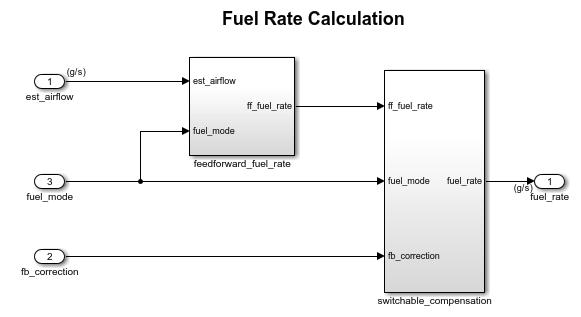
\includegraphics[width=0.7\linewidth]{src/pic/simulink}
    \caption{Simulink schema example.}
    \label{fig:simulink}
\end{figure}

Simulink has plenty of tutorials in many different areas with detailed description and videos on solving it which describes it step-by-step. It is very helpful to have step-by-step solution with detailed description for understanding all important details. Because on this understanding of essentials, is build the future knowledge and depends future success. But there is some weakness in an education process. The issue is, that they don't have methods for validating the correctness of the user's solution and does not encourage the users to try it out by themselves, just copy the sample solution.

\section{Rust} \label{sec:rust}
Rust(Link) is a very popular programming language the prevalence of which is growing every day. It has a consistent tutorial which describes language constructs with gradually increasing complexity. It has the informative and structured index, where users can easily jump from one topic to another almost instantly and then just go back to the place where he was reading before. They use highlighted ares to show some code examples, which facilitate understanding of presented materials. It is possible to copy some parts of the code and even directly execute it in a browser(see figure \ref{fig:rust}).

\begin{figure}[h!]
    \centering
    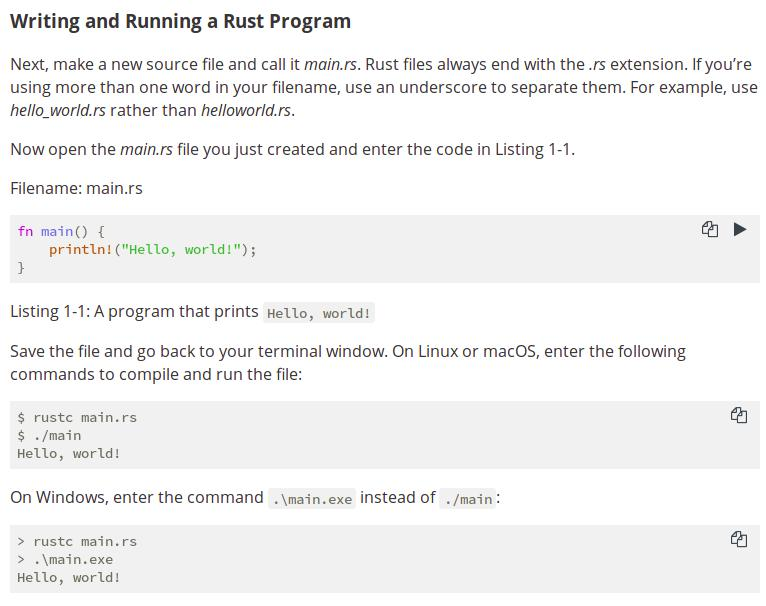
\includegraphics[width=0.7\linewidth]{src/pic/rust}
    \caption{Rust tutorial example.}
    \label{fig:rust}
\end{figure}

To execute the given code, you just have to click on the play button in the upper right corner and in several second the result will be displayed. This is very important and useful feature, because students can directly see what the code does. At the given example it is pretty straightforward, but if you have some computation, not even complex one, it is already not so easy to imagine the output.
Nevertheless, even in this short example, there is some issues related to the compilation process. Namely, the different compilation and execution process for diverse platforms(Windows, Linux, macOS). It means, that we have to install the compiler to use it during the learning process. It would be very convenient to have all these features directly in the web-browser, without installation.

\section{Microsoft Z3 Solver} \label{sec:z3}
Z3 is a state-of-the art theorem prover from Microsoft(link). It provides similar experience compare to Rust tutorial but with some improvements, which simplify the studying process. There is a possibility, not only to execute the given code from the current example directly in the browser, but edit the code, and still see the result almost instantly due to in-browser execution. It helps to see the direct binding between written commands and the real result, that improves understanding of given material.

\begin{figure}[h!]
    \centering
    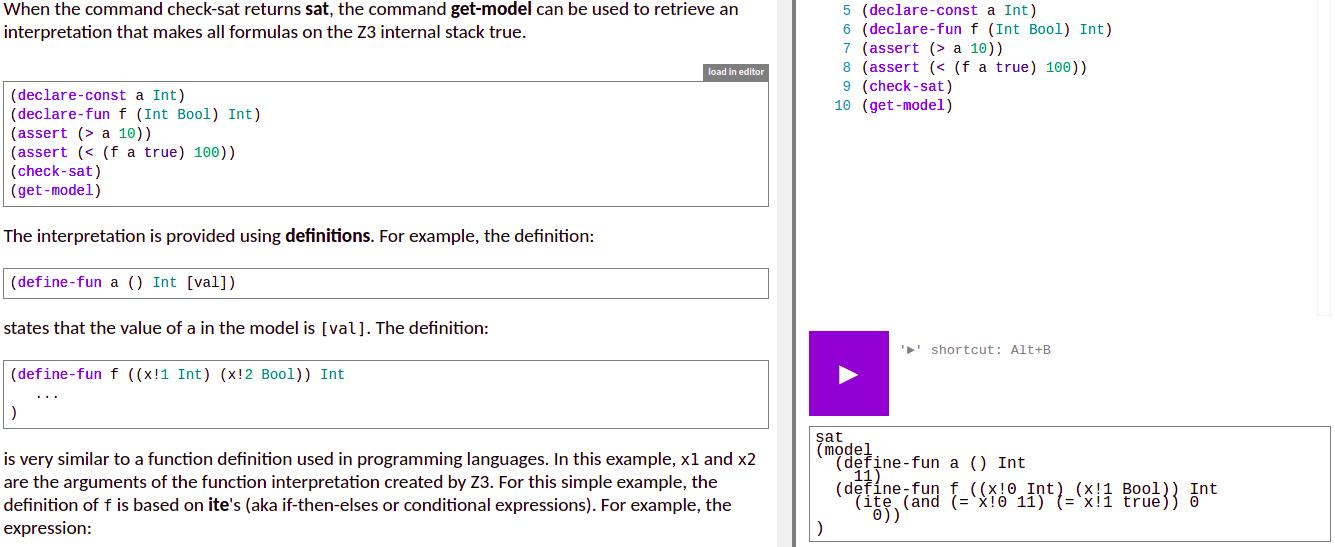
\includegraphics[width=\linewidth]{src/pic/z3}
    \caption{Z3 tutorial example.}
    \label{fig:z3}
\end{figure}

In the figure \ref{fig:z3}, you can see the code given in a tutorial on the left hand side. On the right hand side, there is the code which has been executed and the result appeared below. Then you can adjust the code to check some hypothesis, and instantly see the result. By doing this, students can check their understanding of an explained material.
Another advantage in this tutorial is a in-browser execution. Students do not have to install anything and can directly work in browsers. It means, the operating system(OS) does not have any influence on the execution and compilation process. Any OS can be used, it is necessary to have a web-browser. If this tutorial will be used directly on a lecture, then students just enter the URL in a browser and can instantly try to execute some examples.

\section{Octave Online} \label{sec:octave}
Octave Online(link) is a web-playground fot a high-level language Octave, which is primarily intended for numerical computations. It has a simple and intuitive interface despite the complexity of the internal implementation. It provides directly in a browser fast execution with errors handling. Even if you do complex computations it is not needed to install any software on the PC. Everything works out of the box.

\begin{figure}[h!]
    \centering
    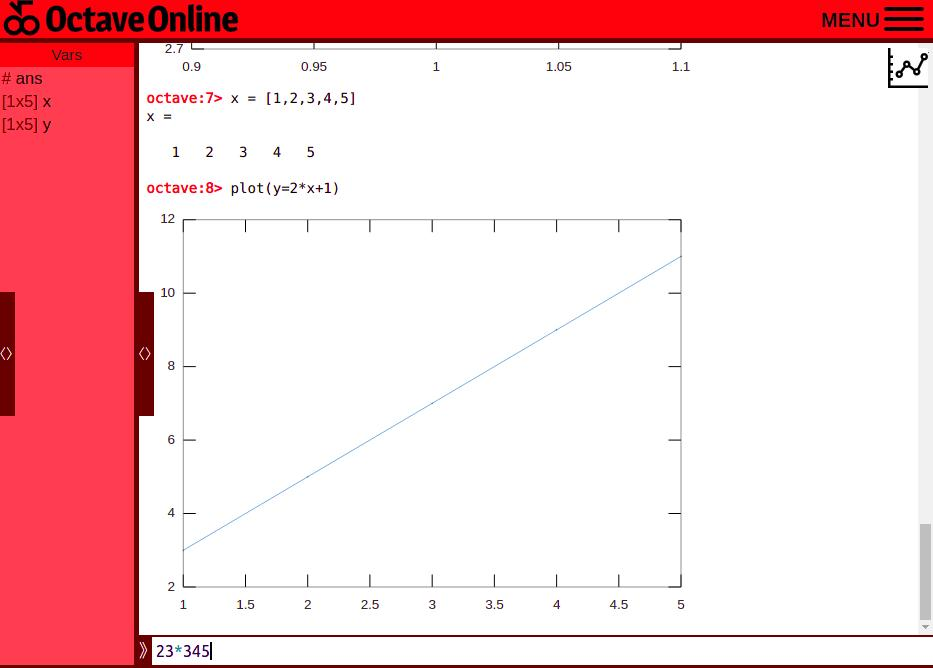
\includegraphics[width=0.7\linewidth]{src/pic/octave}
    \caption{Octave web-playground example.}
    \label{fig:octave}
\end{figure}

This web-playground is oriented on students, who are using the tool directly on the lecture. Do some computations in a browser and run previously created scrips, as a sequence of the commands. To visualize some data, there is a possibility to build some plots for better understanding.

\section{Wolfram Alpha} \label{sec:wolfram}
Wolfram Alpha is a very powerful tool, which works by using expert-level knowledge and algorithms to automatically answer questions, do analysis and generate reports. It has matrix operations and calculations as the EmbeddedMontiArcMath(link) language has, to describe atomic components. It can do even more as solving linear equations, it allows to specify the behavior of controllers, and then, by solving the equations, they synthesize the controller. Furthermore, it has one very interesting and useful feature, which provide the interactive visualization of the given data. The idea behind that is that you can \"feel\" how one or another parameter influence on the final result. It promises a better understanding of the dependencies between the components or elements of the system.

\begin{figure}[h!]
    \centering
    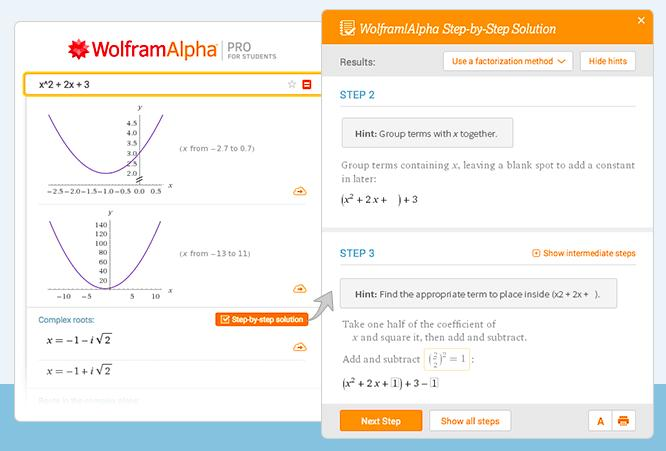
\includegraphics[width=0.7\linewidth]{src/pic/wolfram}
    \caption{Wolfram Alpha example.}
    \label{fig:wolfram}
\end{figure}

It offers the tutorials, which have step-by-step solution with detailed explanation of each step and additional hints for students(see figure \ref{fig:wolfram}). Futhermore, it has high quality visualization, which encourage students to do some experiments and see the changes on the displayed figure.

\section{TypeScript Playground} \label{sec:typescript}
TypeScript is a typed superset of JavaScript. It has a clean and simple playground which shows the difference and benefits of TypeScript over JavaScript. It has preloaded examples which actually show this difference and a user can see distinction in the direct comparison(see figure \ref{fig:typescript}). What, again, gives the better understanding and facilitates further analysis.

\begin{figure}[h!]
    \centering
    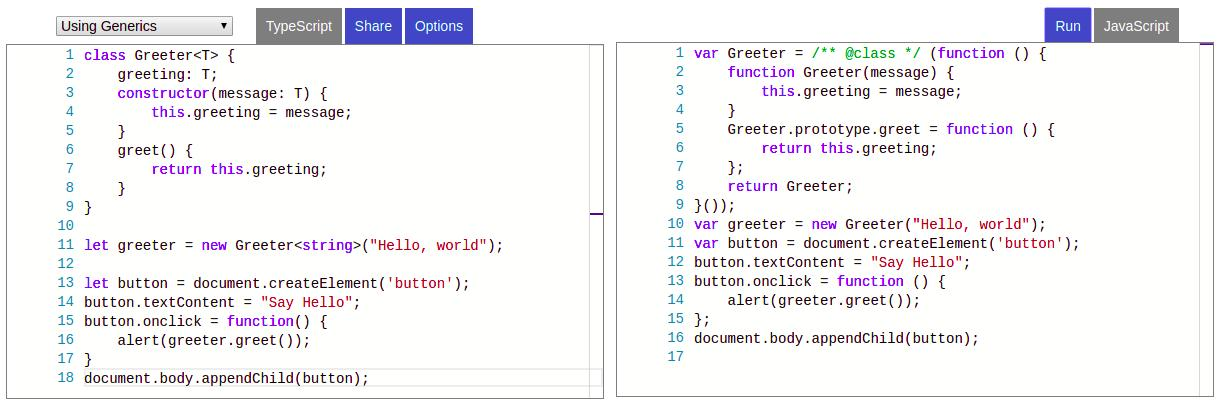
\includegraphics[width=\linewidth]{src/pic/typescript}
    \caption{Typescript playground example.}
    \label{fig:typescript}
\end{figure}

In the picture, it emphasizes the difference in classes architecture. It helps to find architecture advantages of using new language(means Typescript). Moreover, you can run the given example and see the result directly in a browser, but in different tab, which is not really convenient. If you have some complex code, it is really helpful to see the source and the result simultaneously.

\section{Swift Playground} \label{sec:swift}
Swift Playground has been created for teaching the Swift language in a game form. You can create small programs that instantly show the results of the code that you write. From the right side of the screen is shown a 3D world where an action is happen(see figure \ref{fig:swift}). The tutorials are pretty simple but the concept is very interesting. They have automatic verification of an implemented correctness in the 3D environment. To produce many diverse game oriented tutorials, it would be convenient to have simple 3D models importing which can use different models from various 3D editors.

\begin{figure}[h!]
    \centering
    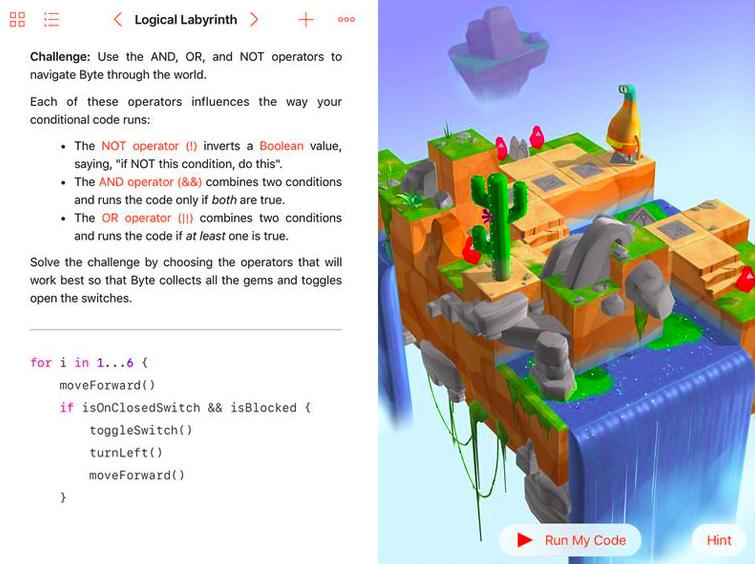
\includegraphics[width=0.6\linewidth]{src/pic/swift}
    \caption{Swift playground example.}
    \label{fig:swift}
\end{figure}

Apple gives into trends and have used the gamification in the tutorials, to attract learners to their product.

\section{Requirements deriving}
Thoroughly analyzed the projects described above, the following list of requirements has been derived: \\\\
(R1) 3D visualization for demonstration purposes \\
(R2) Simple, clean and intuitive interface \\
(R3) Work on any operating system and without installation \\
(R4) Automatic verification of obtained results \\
(R5) Import and use existing 3D models for the simulation \\
(R6) Displaying the object's trajectory \\
(R7) Integrated testing support \\

The table summarizes the comparison between the all considered tutorials. \\
\begin{table}[h!]
    \begin{tabular}{|l|l|l|l|l|l|l|l|l|}
    \hline
    &  Z3 Solver & Octave & Wolfram & TypeScript & Swift & Rust & Simulink & EMAM PG \\ \hline
    R1 & - & + & + & - & + & - & + & + \\ \hline
    R2 & + & + & + & + & + & + & + & + \\ \hline
    R3 & + & + & + & + & - & + & - & + \\ \hline
    R4 & - & - & - & - & + & - & + & + \\ \hline
    R5 & - & - & - & - & - & - & + & + \\ \hline
    R6 & - & - & P & - & P & - & P & + \\ \hline
    R7 & - & - & - & - & - & - & + & + \\ \hline
    \end{tabular}
\end{table}
(+ support, P partially support) \\

Take a closer look at the differences between the tutorials regarding to the derived requirements.\\
(R1) 3D visualization for demonstration purposes: Four considered tutorials have a 3D visualization. The Octave online has a possibility to generate plots and graphics for given data. The Wolfram Alpha has a very powerful tool which can generate 3D models and you can even interact with them and see the changes in a real time. Whereas the Swift Playground has the most advanced 3D world which is like a part of the tutorial and result presentation. The Simulink has an opportunity to build nice 3D models which involved in the simulation process, but the difference is that a user has to build everything himself.\\
(R2) Simple, clean and intuitive interface: This is the only requirement which all tutorial are satisfied. We believe that it is very important to have an understandable and clear interface which does not distract from the educational process. Moreover, the interface should be intuitive so that students can use it directly at the lecture without detailed explanation of its features. \\
(R3) Work on any operating system and without installation: Almost all examined tutorials have web-implementation and work without installation, except the Swift tutorial and Simulink. The Swift tutorial has only iOS implementation. The Simulink does not work on the Web too, only the MathLab, which has partial web-implementation.\\
(R4) Automatic verification of obtained results: Only one among the examined tutorials, the Swift tutorial, has a gaming base verification of a solution correctness. It causes additional interest in the studying process, and can be the motivation to keep solving the tasks, by analogy with computer games. Whereas the Simulink gives you possibility to do it, but it is more like extra feature which can be implemented.\\
(R5) Import and use existing 3D models for the simulation: Only the Simulink has feasibility to import 3D models. It helps to create tutorials quickly and efficiently, by using the previously created models and configurations. An example of reusing a 3D object can be a cone that is used in many exercises. This feature simplifies the process of creating new tutorials and decreases the time which has to be invested into the building process.\\
(R6) Displaying the object's trajectory: Wolfram Alpha, Swift PG and Simulink, we could say, partially support this feature in case that you can see the whole process of movement of the object from the very beginning to the end. But it would be better to improve the concept and add the separate window which permanently displays a traversed route of the object, for better visual perception and visual comparison of results. In our case the object is a car.\\
(R7) Integrated testing support: Only the Simulink has integrated testing options. Due to the specificity of the tutorials, tests play an important role. Writing the streaming test for components, students can be sure that it reacts properly to the incoming data. Tests make the components more reliable and robust. Because of the using the C\&C language, it is great to be sure that each component of a composed model behaves correctly.  
Taking into account all these derived requirements we going to start working on the architecture.\\

\cleardoublepage

\chapter{Preliminaries}
The section introduces technologies that have been used in this thesis. The section \ref{sec:ema} gives an overview of the modelling C\&C language - EmbeddedMontiArc(EMA). The section \ref{sec:tools} presents the whole stack of EmbeddedMontiArc tools that have been used in the toolchain. More detailed description of the tools will be given in the following subsections: the subsection \ref{sec:emam2wasm} EMAM2Wasm describes the generator, which translate code from the EmbeddedMontiArcMath(EMAM) to C++ and then to Web-assembly. The subsection \ref{sec:onlineide} gives an overview of the Online IDE, which is used for writing EMA code in a browser. The subsection \ref{sec:svggen} explains the features of the schema' picture generator.
\section{EmbeddedMontiArc language} \label{sec:ema}
EmbeddedMontiArc language belongs to the MontiCAR language(link) family. It was designed to model architectures of embedded and cyber-physical systems. To show the main advantages of the language, it is easier to start directly with the example \ref{fig:embdmontiarc}.
\begin{figure}[h!]
    \centering
    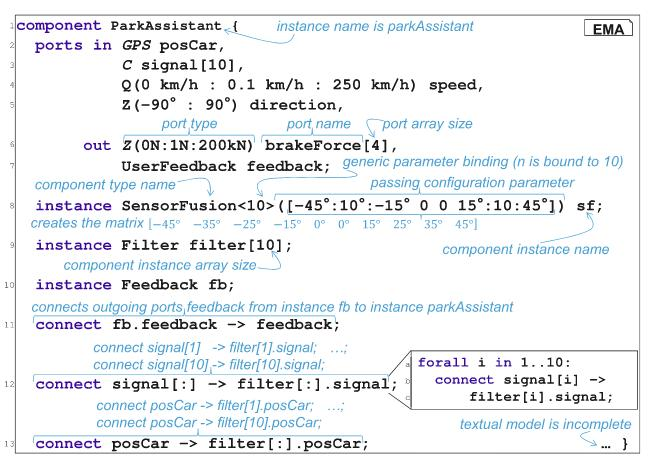
\includegraphics[width=\linewidth]{src/pic/embdmontiarc}
    \caption{Textual EmbeddedMontiArc model of ParkAssistant.}
    \label{fig:embdmontiarc}
\end{figure} \\
In the picture is shown the component with the name - ParkAssistant. This is not the entire component but a main part, which shows the most important features. It has incoming and outgoing ports. All ports must have a type, name and range. The type defines a kind of a signal(e.g., Q,N,Z,B). The range is very important, it helps to control the signal in boundaries, which are defined in advance. Moreover, the range defines not only the boundary values, but the units(e.g., km/h, m/s and so on). Another option, which is available for ports - port size array. It is possibility to define an array of ports, it can increase the readability of the connection schema and simplify the ports connection. When the component is created and ports have been defined, it is possible to instantiate another components inside the component. How you can seen in the lines 8,9 and 10, there are several features available. The first one is to define the generic parameter for a component, to be able create a more general component, which can be used for different types of incoming signal. The next one is to create an array of components, if it is required several similar components for some reason, like the filter component, which does some signal refining. The last one, it is just a normal component instantiation, without any extra parameters. When all required components have been instantiated, it is time to connect the components together. EmbeddedMontiArc offers several convenient options to do that. Firstly you can just connect the specific port of one component to another specific port of another component, like it is shown in the 11th line. Then it is possible to connect an array of ports to another one, to reduce the number of connections between components. Another possibility to connect one port of some component to a specific port of other components, like one-to-many connection. 

\section{EMA Tools} \label{sec:tools}
In this section will be described a full stack of components, which have been used in the toolchain. These components have been developed by other students and in this thesis they will be combined in one chain. The first one is Online IDE, which is used in front end, and another two are EMAM2Wasm generator and SVG generator, which are used in the back end.
\subsection{Online IDE} \label{sec:onlineide}
Online IDE is based on the Cloud9 IDE, that is an online integrated development environment. It supports various languages and was adapted to support the EmbeddedMontiArc and EmbeddedMontiArcMath. It has many features which simplify the development process(see figure \ref{fig:onlineIDE}). The IDE supports the autocompletion for the given languages and syntax highlighting. It increases the speed of the development process and convenience during the code writing. From the left hand side is located the directory tree, which is simplify the navigation inside the project. In this area, you can create new files and folders. Files, which have beed opened, organized in tabs, which can be also used for navigation. From the right hand side, there is shown the list of all ports of the currently selected component. Then the list of the sub-components, which contains the selected component. It shows types of components and their names. When there are many other components in the component, it is easier to see the entire list of components in one screen. Below the sub-components, a group of connectors is shown, which are used to connect currently selected component with others components instantiated inside it. Moreover, the autocompletion is offered to connect to ports of a component, which actually has this component. It means that, the autocompletion tracks all instantiated components with ports. Needless to say, that the IDE supports a text search and search through the ports, sub-components and connectors.
\begin{figure}[h!]
    \centering
    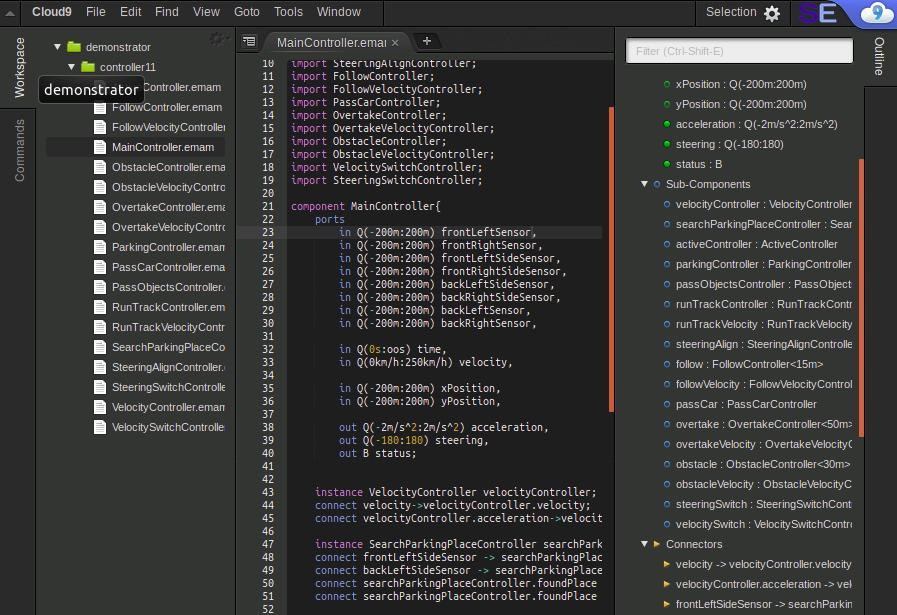
\includegraphics[width=\linewidth]{src/pic/onlineIDE}
    \caption{EMA Online IDE.}
    \label{fig:onlineIDE}
\end{figure} \\
To store porject's files, a virtual file system(VFS)(link) is used. It provides the filesystem API, which is used by developers to manipulate the project's files. It makes available all basic methods for working with files and folders(e.g., mkdir, readFile, copy and so on).
\subsection{EMAM2Wasm} \label{sec:emam2wasm}
This tool generates the web-assembly binary file and JavaScript file from the EMA project. The tool is based on the EMAM2Cpp generator, which firstly produces the c++ equivalent of the EMAM model, afterwards the generated c++ model is used to generate the Web-assembly model, using Emscripten compiler \cite{Emscripten}. The produced files later are used in a browser to execute compiled EMA model for the 3D visualization process. \\
The tool is consisted of the .jar file, which has packed with all dependencies and script files. One of these script files, does the setup procedure and another one executes the main .jar file, with all important parameters. One of the important parameters, which is given in the script file, is a path to Armadillo \cite{Armadillo} library. It is a C++ library for linear algebra \& scientific computing and it is used for matrix computations.
\subsection{SVG generator} \label{sec:svggen}
The main purpose of the SVG generator to create single or multiple layers schema of the given controller. The generated schema helps to visualize the textual model of the EMA controller. The visualization can help to find some errors related to incorrect connection between some components. The SVG generator able to generate multiple layer models, that increases a readability of schemas, because firstly you see more general schema of the model, then you just need to click on some component and an internal schema of the component is appeared.
\begin{figure}[h!]
    \centering
    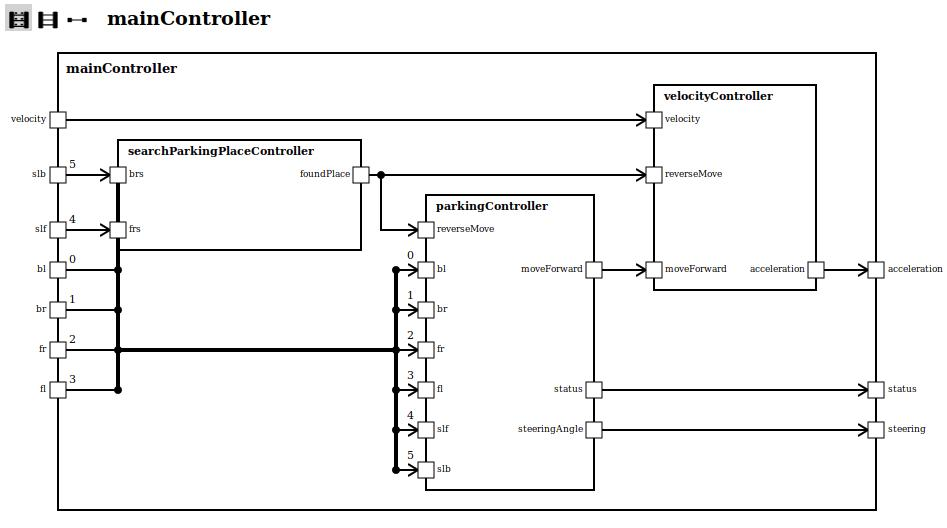
\includegraphics[width=\linewidth]{src/pic/controller03}
    \caption{EMA Parking controller.}
    \label{fig:parking}
\end{figure}
In the figure \ref{fig:parking} is depicted the parking controller, which has three internal sub-components. Each of these components can have another components inside. The generator calculates the layout in the way to optimize positions of components and decrease the length of the connectors between them. One of the features, is a possibility to simplify the schema by hiding the ports' names and grouping the connections between components.
\chapter{Tutorials}
In this chapter a group of tutorials will be presented. The goal of the tutorials to teach students the basics of the EmbeddedMontiArc language and give a general idea how to build the autopilot's models. The tutorials are given with respect of an increasing the complexity level. Examples are explained step-by-step, to give the best studying experience.
\section{Zero tutorial}
\textbf{Task:} accelerate to the given speed. \newline
Implement the model that continuously accelerates to 10 m/s and then stops.\\ \\
Basic explanation:\\
The car has 8 sensors to measure distances to obstacles. They are located respectively: \\
\begin{figure}[h!]
    \centering
    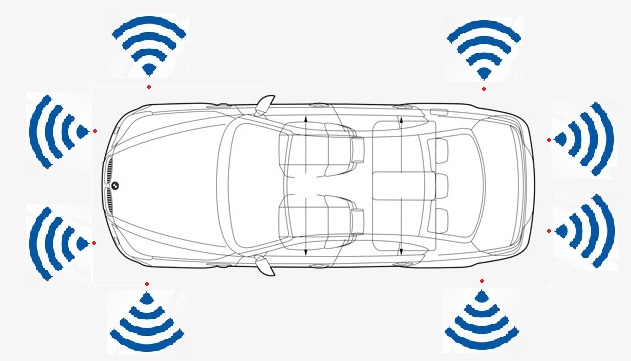
\includegraphics[width=\linewidth]{src/pic/car-with-sensors}
    \caption{Car with sensors.}
    \label{fig:sensors}
\end{figure} \\
To solve this task it's needed to control only an acceleration of the car. Changing the acceleration you may control the behavior of the car. To be able to reach 10 m/s speed, you have to accelerate the car continuously until it reaches the desired speed. Let's start with a MainController which defines the interface to the simulator. We should create a new file which has the same name like component has, with .emam extension.
\bigskip
\begin{lstlisting}
    package controller;

    component MainController{
        ports                                   
            in Q(-200m:200m) frontLeftSensor,
            in Q(-200m:200m) frontRightSensor,
            in Q(-200m:200m) frontLeftSideSensor,
            in Q(-200m:200m) frontRightSideSensor,
            in Q(-200m:200m) backLeftSideSensor,
            in Q(-200m:200m) backRightSideSensor,
            in Q(-200m:200m) backLeftSensor,
            in Q(-200m:200m) backRightSensor,
    
            in Q(0s:oos) time,
            in Q(0m/s:25m/s) velocity,
            in Q(-200m:200m) xPosition,
            in Q(-200m:200m) yPosition,
    
            out Q(-2m/s^2:2m/s^2) acceleration,
            out Q(-180 deg:180 deg) steering,
            out B status;
    ...
\end{lstlisting}
\bigskip
The first eight incoming ports, lines from 5 to 12, receive the data from the sensors which are shown in the picture \ref{fig:sensors}. The next port is a simulation time, which starts from zero second to infinity. The velocity incoming port shows a current velocity of the car. And the next two ports give a position of the car on a track. After the incoming ports the outgoing are following. Outgoing ports control a behaviour of the car using the data which is coming to the incoming ports. The acceleration port controls the velocity, it is like you have two pedals in the car. If you push a brake, you have a negative acceleration. But if you push an accelerator pedal, the car accelerates and velocity has been increased. Then following the steering port, which controls the rotation of the car. And finally the status port, which signals the end of a simulation process. The reason to finish the simulation can be a successful completion of an assignment or violating by the car the track or a map borders. \\
After examination of the example, we should notice:
\begin{itemize}
\item Component has ports incoming and outgoing
\item For each port must be specified a type ( like Q,B) with a valid range.
\item After each port name has to be a comma and the last one must have a semicolon.
\item The possible units are:
    \begin{itemize}
        \item Distance: meters(m), kilometers(km)
        \item Time: seconds(s), minutes(m), hours(h)
        \item Velocity: km/h, m/s
        \item Acceleration: m/s\^2
        \item Rotation: degrees(deg)
    \end{itemize}
\end{itemize}
It was the default interface for the Simulator. It has to be define for all feature controllers. Then you should create your own components which will be connected to the mainController. Let's create a simple component and connect it to the main one. To do that, we have to create a new file .emam with the following content:
\bigskip
\begin{lstlisting}
    package controller;

    component ExampleController {
	    ports
		    in Q(0m/s : 25m/s) velocity,
		    out Q(-2m/s^2:2m/s^2) acceleration,
		    out B status;

	    implementation Math{
		
		    if (velocity <= 10 m/s)
    	        acceleration = 1m/s^2;
    	    else
    	    	status = true;
            end
	    }
    }
\end{lstlisting}
\bigskip
In this component, which is named - ExampleController, are one incoming port and two outgoing ones. Firstly we should reach the speed 10 m/s then stop the simulation. The logic of the controller is implemented inside the Math{} scope. Inside the Math scope you can see if-else-end constructions and the example how to use it. Moreover, it the Math scope can be used different constructions, which you will see later in the next tutorials. The logic in this controller pretty straightforward, it the velocity of the car is less then 10 m/s then accelerate the car with the acceleration 1 m/s. When the given velocity is reached, stop the simulation by setting the status port to true. \\
When we have created the ExampleController we should import it into the MainController and then instantiate it, to have possibility to use it, like a part of the MainController:
\bigskip
\begin{lstlisting}
    package controller;

    import ExampleController;

    component MainController{ 
    ...

    instance ExampleController exampleController;
    ...
\end{lstlisting}
\bigskip
How you can see, we have imported the ExampleController in the line 3. Then later, after specifying the ports of the MainController we have instantiate the controller with the type ExampleController and the name exampleController. Now we should connect this controller to the main controller using specified ports.
\bigskip
\begin{lstlisting}
    ...
    connect velocity->exampleController.velocity;
    connect exampleController.acceleration->acceleration;
    connect exampleController.status->status;
}
\end{lstlisting}
\bigskip
We have connected the incoming port - velocity(mainController) to our instantiated controller and it's corresponding incoming port velocity. Then we connected the outgoing port of velocityController.acceleration to the outgoing port of our MainController. And finally the status port of the ExampleController to status of the MainController.\\
Finally the connections scheme should look like is depicted in the figure \ref{fig:controller}.
\begin{figure}[h!]
    \centering
    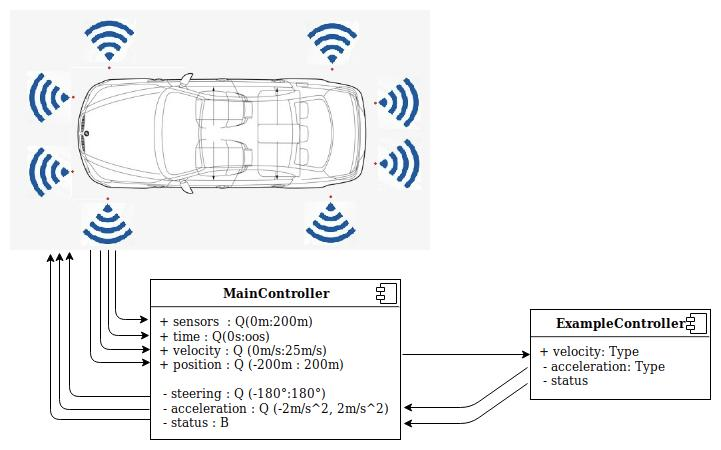
\includegraphics[width=\linewidth]{src/pic/car-with-controller}
    \caption{Car with controller.}
    \label{fig:controller}
\end{figure} \\
Eventually we should send these files to the server to process it and then execute in the simulator, to the how the car behaves using our first controller.
\section{Parallel parking tutorial}
\textbf{Task:} To carry out a parallel parking between two cars. \newline
Implement a model that manages a parking between two cars. The model has to have several modules which are responsible for different actions. One of the examples could be:
\begin{enumerate}
    \item Module which controls the speed of the car, depends on the current action(e.g. parking, searching a parking place).
    \item Module which looking for a gap between cars for the parking.
    \item Module which controls a steering of the car during the parking process.
\end{enumerate}
Each module should be as simple as possible. \newline
To solve this task you should use at least 6 sensors, which measure the distance to objects which are located in front, left side and back of the car. The speed has to be around 0.5-1 m/s. In the picture you can see the main idea how the parking has to be done:
\begin{figure}[h!]
    \centering
    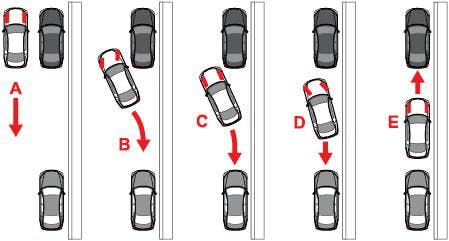
\includegraphics[width=0.8\linewidth]{src/pic/parking_process1}
    \caption{Parking process.}
    \label{fig:parking}
\end{figure}
The parking process can be divided in 4 steps:
\begin{enumerate}
    \item Go straight until a place have been found.
    \item When the place is found, go back and rotate the car.
    \item When the car has reached appropriate point, rotate car in other direction to fit into given gap between the cars.
    \item When the car is close to the car behind, stop and go forward until it reaches certain distance to the front car.
\end{enumerate}
Important to know, this wed-simulator is a simplified version and it does not change the angle of front wheels but an angle of the car entirely. \newline \newline
\textbf{Solution} \newline \newline
To solve that tutorial we have to use the MainController, like we did in the previous tutorial. But we are going to start from an implementation of a controller which will search the place for the car, between two other cars to carry out the parallel parking. The idea is to pass the first car and find the "end" of the second car to start parking process form a right point, like it is shown in the picture \ref{fig:parking}.
\bigskip
\begin{lstlisting}
package controller03;

component SearchParkingPlaceController {
    port
        in Q(-200m:200m) frontLeftSide,
        in Q(-200m:200m) backLeftSide,
        out B foundPlace;

    implementation Math{
        
        static Q passed0 = false;
        static Q passed1 = false;
        static Q passed2 = false;
        static Q passed3 = false;

        if ((backLeftSide - frontLeftSide) > 3m)
            passed0 = true;
        end

        if (((frontLeftSide - backLeftSide) > 3m) && passed0)
            passed1 = true;
        end
        
        if (((backLeftSide - frontLeftSide) > 3m) && passed1)
            passed2 = true;
        end
        
        if (((frontLeftSide - backLeftSide) > 3m) && passed2)
            passed3 = truetutorials/controllers/controller03/SearchParkingPlaceController.emam;
        end
        
        foundPlace = passed3;
    }
}    
\end{lstlisting}
\bigskip
We are using the side sensors to measure the distances to the cars and the side of the road. Using static variables we can save the states(e.g. the distance has changed from 5m to 1m and then from 1m to 5m, it means we have passed the car). Static variables initialized only once. Now we should create a VelocityController, which controls the speed of the car, during the search parking place process and parking.
\bigskip
\begin{lstlisting}
    package controller03;

    component VelocityController {
        port                                    
            in Q(0km/h : 250km/h) velocity,
            in B reverseMove,
            in B moveForward,
            out Q(-2m/s^2:2m/s^2) acceleration; 
    
        implementation Math{                    
    
            if (velocity > 1 m/s)
                acceleration = 0m/s^2;
            else
                acceleration = 1m/s^2;
            end
            
            if reverseMove
                acceleration = -0.5 m/s^2;
            end
            
            if (velocity < -0.5 m/s)
                acceleration = 0m/s^2;
            end
            
            if (reverseMove && moveForward)
                acceleration = 0.5 m/s^2;
            end
            
            if (reverseMove && moveForward && (velocity > 0.5 m/s))
                acceleration = 0m/s^2;
            end
        }
    }
\end{lstlisting}
\bigskip
The velocityController has several different states. The first one is a limit for the velocity during searching parking place (1m/s). The next one is the velocity limit during the reverse move, -0.5 m/s it means, that car moves back. The last one, when the car moves forward during the parking process to move closer to the front car. Next controller will be the most important one, because it manages the parking process.
\bigskip
\begin{lstlisting}
package controller03;
component ParkingController {
    port
        in Q(-200m:200m) frontLeftSensor,
        in Q(-200m:200m) frontRightSensor,
        in Q(-200m:200m) frontLeftSideSensor,
        in Q(-200m:200m) backLeftSideSensor,
        in Q(-200m:200m) backLeftSensor,
        in Q(-200m:200m) backRightSensor,
        in B reverseMove,
        out Q(-35deg:35deg) steering,
        out B moveForward,
        out B status;

    implementation Math{
        
        static B forwardState = false;
        
        if reverseMove
            steering = 1 deg;
        else
            steering = 0 deg;
        end
        
        if (reverseMove && (backLeftSensor < 2m))
            steering = -1 deg;
        end
        
        if (reverseMove && ((backRightSensor == backLeftSensor) ||
            ((backRightSensor < 3m) && (backLeftSensor < 3m))))
                forwardState = true;
        end
        
        if (((frontRightSensor < 3m) || (frontLeftSensor < 3m)) &&
            forwardState)
            status = true;
        else
            status = false; 
        end
        
        if(forwardState &&(frontLeftSideSensor > backLeftSideSensor))
            steering = -0.5 deg;
        end
        
        if(forwardState &&(frontLeftSideSensor < backLeftSideSensor))
            steering = 0.5 deg;
        end
        
        moveForward = forwardState;
    }
}
\end{lstlisting}
\bigskip
The idea is that the car is going back until it reached a certain point, changing an angle of the car. When the car is going back and a distance, from the back left sensor to the road border, is less then 2m, start rotate the car in opposite direction until it is in parallel with the road. Then stop when the limit of the back distance is reached and get closer to the front car. All these steps are nicely illustrated in the picture \ref{fig:parking}. Finally we should connect all these controllers to the interface in the MainController.
\bigskip
\begin{lstlisting}
    package controller03;

    import VelocityController;
    import SearchParkingPlaceController;
    import ParkingController;
    
    component MainController{
        ports 
            in Q(-200m:200m) frontLeftSensor,
            in Q(-200m:200m) frontRightSensor,
            in Q(-200m:200m) frontLeftSideSensor,
            in Q(-200m:200m) frontRightSideSensor,
            in Q(-200m:200m) backLeftSideSensor,
            in Q(-200m:200m) backRightSideSensor,
            in Q(-200m:200m) backLeftSensor,
            in Q(-200m:200m) backRightSensor,
    
            in Q(0s:oos) time,
            in Q(0km/h:250km/h) velocity,
    
            in Q(-200m:200m) xPosition,
            in Q(-200m:200m) yPosition,
    
            out Q(-2m/s^2:2m/s^2) acceleration,
            out Q(-180deg:180deg) steering,
            out B status;
    
        instance VelocityController velocityController;
        connect velocity->velocityController.velocity;
        connect velocityController.acceleration->acceleration;
    
        instance SearchParkingPlaceController searchParkingPlace;
        connect *->searchParkingPlace.*;
        
        instance ParkingController parkingController;
        connect *->parkingController.*;
        connect searchParkingPlace.foundPlace-> [
            velocityController.reverseMove,
            parkingController.reverseMove];
        connect parkingController.*->*;
        connect parkingController.*->velocityController.*;
    }
\end{lstlisting}
\bigskip
All Controllers have been instantiated and then connected to the corresponding ports. The star on the line 33 and later means that the ports, which have similar name are connected to each other. The entire connection scheme is depicted in the figure \ref{fig:parking-scheme}.
\begin{figure}[h!]
    \centering
    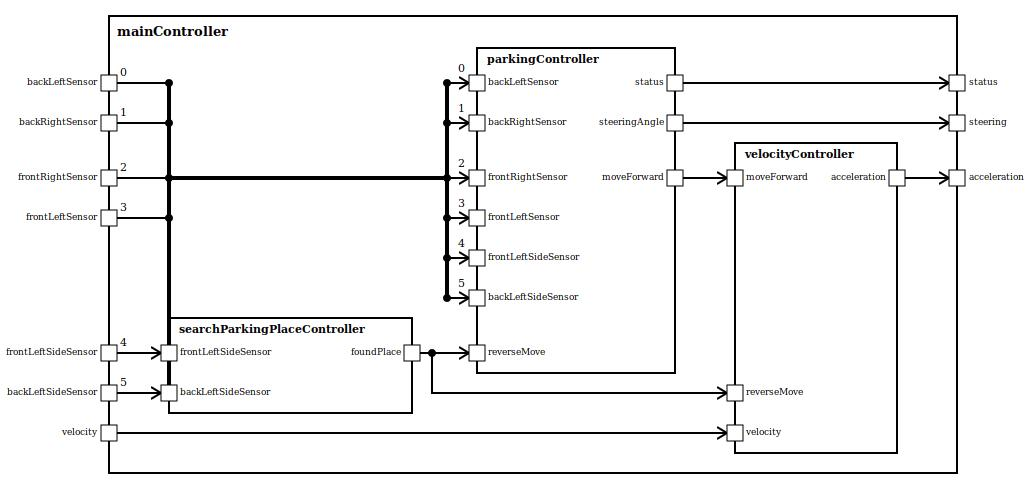
\includegraphics[width=\linewidth]{src/pic/parking-scheme}
    \caption{Parking controller scheme.}
    \label{fig:parking-scheme}
\end{figure}
\section{Maneuverability test tutorial}

\chapter{Toolchain implementation}
\section{3D web-simulator}
\section{Client-side}
\section{Server-side}
\section{CoCo checker}
